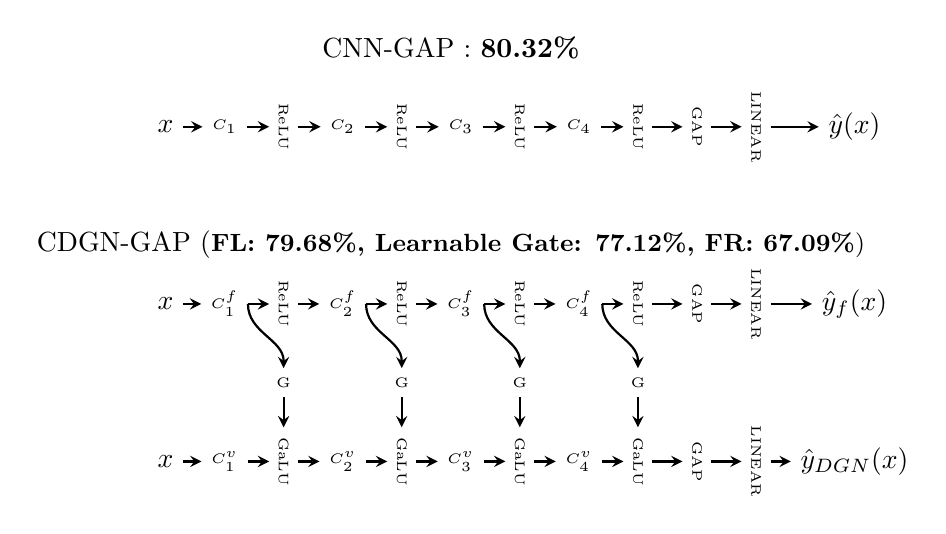
\begin{tikzpicture}
\node []  (dnn-text)at (4.125,2) {CNN-GAP : \textbf{80.32\%}};

\node []  (dnn-output) at (9.25,1) {$\hat{y}(x)$};
\node [rotate=-90]  (dnn-smax) at (8,1) {\tiny{LINEAR}};
\draw [-stealth,thick]   (dnn-smax.north) -- (dnn-output.west);

\node [rotate=-90]  (dnn-gap) at (7.25,1) {\tiny{GAP}};
\draw [-stealth,thick]   (dnn-gap.north) -- (dnn-smax.south);

\node [rotate=-90] (dnn-relu-4) at (6.5,1){\tiny{ReLU}};
\node [] (dnn-c4) at (5.75,1){\tiny{$C_4$}};
\draw [-stealth,thick]   (dnn-c4.east) -- (dnn-relu-4.south);
\draw [-stealth,thick]   (dnn-relu-4.north) -- (dnn-gap.south);



\node [rotate=-90] (dnn-relu-3) at (5,1){\tiny{ReLU}};
\node [] (dnn-c3) at (4.25,1){\tiny{$C_3$}};
\draw [-stealth,thick]   (dnn-c3.east) -- (dnn-relu-3.south);
\draw [-stealth,thick]   (dnn-relu-3.north) -- (dnn-c4.west);


\node [rotate=-90] (dnn-relu-2) at (3.5,1){\tiny{ReLU}};
\node [] (dnn-c2) at (2.75,1){\tiny{$C_2$}};
\draw [-stealth,thick]   (dnn-c2.east) -- (dnn-relu-2.south);
\draw [-stealth,thick]   (dnn-relu-2.north) -- (dnn-c3.west);

\node [rotate=-90] (dnn-relu-1) at (2,1){\tiny{ReLU}};
\node [] (dnn-c1) at (1.25,1){\tiny{$C_1$}};
\draw [-stealth,thick]   (dnn-c1.east) -- (dnn-relu-1.south);
\draw [-stealth,thick]   (dnn-relu-1.north) -- (dnn-c2.west);



\node [] (dnn-input) at (0.5,1){$x$};
\draw [-stealth,thick]   (dnn-input.east) -- (dnn-c1.west);


%%%%%%%%%%%%%%%%%%%%%%%%%%%%%%%%%%%%%%%%%%%%%%%%%%%%%%%%%%%%%%%%%
\node []  (fntext)at (4.125,-.5) {CDGN-GAP (\small{\textbf{FL: 79.68\%, Learnable Gate: 77.12\%, FR: 67.09\%}})};

%\node []  (output) at (7.5,1.5) {$\hat{y}(x)$};


\node [align=right]  (dgn-f-output) at (9.25,-1.25) {$\hat{y}_{\text{f}}(x)$};
\node [rotate=-90]  (dgn-f-smax) at (8,-1.25) {\tiny{LINEAR}};
\draw [-stealth,thick]   (dgn-f-smax.north) -- (dgn-f-output.west);

\node [rotate=-90]  (dgn-f-gap) at (7.25,-1.25) {\tiny{GAP}};
\draw [-stealth,thick]   (dgn-f-gap.north) -- (dgn-f-smax.south);


\node [rotate=-90] (dgn-relu-4) at (6.5,-1.25){\tiny{ReLU}};
\node [] (dgn-f-c4) at (5.75,-1.25){\tiny{$C^{\text{f}}_4$}};
\draw [-stealth,thick]   (dgn-f-c4.east) -- (dgn-relu-4.south);
\draw [-stealth,thick]   (dgn-relu-4.north) -- (dgn-f-gap.south);


\node [rotate=-90] (dgn-relu-3) at (5,-1.25){\tiny{ReLU}};
\node [] (dgn-f-c3) at (4.25,-1.25){\tiny{$C^{\text{f}}_3$}};
\draw [-stealth,thick]   (dgn-f-c3.east) -- (dgn-relu-3.south);
\draw [-stealth,thick]   (dgn-relu-3.north) -- (dgn-f-c4.west);


\node [rotate=-90] (dgn-relu-2) at (3.5,-1.25){\tiny{ReLU}};
\node [] (dgn-f-c2) at (2.75,-1.25){\tiny{$C^{\text{f}}_2$}};
\draw [-stealth,thick]   (dgn-f-c2.east) -- (dgn-relu-2.south);
\draw [-stealth,thick]   (dgn-relu-2.north) -- (dgn-f-c3.west);


\node [rotate=-90] (dgn-relu-1) at (2,-1.25){\tiny{ReLU}};
\node [] (dgn-f-c1) at (1.25,-1.25){\tiny{$C^{\text{f}}_1$}};
\draw [-stealth,thick]   (dgn-f-c1.east) -- (dgn-relu-1.south);
\draw [-stealth,thick]   (dgn-relu-1.north) -- (dgn-f-c2.west);



\node [] (dgn-f-input) at (0.5,-1.25){$x$};
\draw [-stealth,thick]   (dgn-f-input.east) -- (dgn-f-c1.west);

\node [align=right]  (dgn-output) at (9.25,-3.25) {$\hat{y}_{\text{DGN}}(x)$};
\node [rotate=-90] (dgn-smax) at (8,-3.25){\tiny{LINEAR}};
\draw [-stealth,thick]   (dgn-smax.north)--(dgn-output.west);

\node [rotate=-90] (dgn-gap) at (7.25,-3.25){\tiny{GAP}};
\draw [-stealth,thick]   (dgn-gap.north)--(dgn-smax.south);



\node [rotate=-90] (dgn-galu-4) at (6.5,-3.25){\tiny{GaLU}};
\draw [-stealth,thick]   (dgn-galu-4.north) -- (dgn-gap.south);

\node [] (dgn-v-c4) at (5.75,-3.25){\tiny{$C^{\text{v}}_4$}};
\draw [-stealth,thick]   (dgn-v-c4.east) -- (dgn-galu-4.south);

\node [rotate=-90] (dgn-galu-3) at (5,-3.25){\tiny{GaLU}};
\node [] (dgn-v-c3) at (4.25,-3.25){\tiny{$C^{\text{v}}_3$}};
\draw [-stealth,thick]   (dgn-v-c3.east) -- (dgn-galu-3.south);
\draw [-stealth,thick]   (dgn-galu-3.north) -- (dgn-v-c4.west);



\node [rotate=-90] (dgn-galu-2) at (3.5,-3.25){\tiny{GaLU}};
\node [] (dgn-v-c2) at (2.75,-3.25){\tiny{$C^{\text{v}}_2$}};
\draw [-stealth,thick]   (dgn-v-c2.east) -- (dgn-galu-2.south);
\draw [-stealth,thick]   (dgn-galu-2.north) -- (dgn-v-c3.west);


\node [rotate=-90] (dgn-galu-1) at (2,-3.25){\tiny{GaLU}};
\node [] (dgn-v-c1) at (1.25,-3.25){\tiny{$C^{\text{v}}_1$}};

\draw [-stealth,thick]   (dgn-v-c1.east) -- (dgn-galu-1.south);
\draw [-stealth,thick]   (dgn-galu-1.north) -- (dgn-v-c2.west);




\node [] (dgn-input) at (0.5,-3.25){$x$};
\draw [-stealth,thick]   (dgn-input.east) -- (dgn-v-c1.west);




\node[] (dgn-gating-1) at (2,-2.25){\tiny{G}};
\draw [-stealth,thick]   (dgn-f-c1.east) to[out=-90,in=90] (dgn-gating-1.north);
\draw [-stealth,thick]   (dgn-gating-1.south) -- (dgn-galu-1.west);


\node[] (dgn-gating-2) at (3.5,-2.25){\tiny{G}};
\draw [-stealth,thick]   (dgn-f-c2.east) to[out=-90,in=90] (dgn-gating-2.north);
\draw [-stealth,thick]   (dgn-gating-2.south) -- (dgn-galu-2.west);



\node[] (dgn-gating-3) at (5,-2.25){\tiny{G}};
\draw [-stealth,thick]   (dgn-f-c3.east) to[out=-90,in=90] (dgn-gating-3.north);
\draw [-stealth,thick]   (dgn-gating-3.south) -- (dgn-galu-3.west);


\node[] (dgn-gating-4) at (6.5,-2.25){\tiny{G}};
\draw [-stealth,thick]   (dgn-f-c4.east) to[out=-90,in=90] (dgn-gating-4.north);
\draw [-stealth,thick]   (dgn-gating-4.south) -- (dgn-galu-4.west);

	
\end{tikzpicture}

